\chapter{Detector commissioning}
\label{sec:commissioning}

By the end of $2019$, the commissioning of the SuperNEMO demonstrator has begun.
First calorimeter commissioning data were taken.\\
To clatify, we give some common terms used in the detector assembly.
The calorimeter of SuperNEMO is segmented in $712$ optical modules, each composed by the coupling of a photomultiplier tube (PMT for short) and a polystyrene scintillator (see sec.~\ref{sec:calorimeter}).
The divider of a PMT is connected to $2$ cables, one providing the high voltage (HV), the other one, called signal cable, collecting the charge provided by the PMT.
By the summer $2020$, the SuperNEMO demonstrator will be encapsulated in an anti radon tent (\textcolor{red}{abbrev?}).
The so called \emph{patch panel} (PP) will insure passage of cables from inside to outside the anti radon tent, doubling the amount of cables needed for the calorimeter.
We commonly talk about \emph{internal} cables (from detector to patch panel) and \emph{external} cables (from patch panel to electronics).
Consequently, regarding only the calorimeter part, 2848 cables were cut, connector-mounted, transported and installed at Modane.
Then checking cable condition is unavoidable.

\emph{Reflectometry} tests were performed at Modane to check the condition of signal cables:
electronic pulses are generated at electronic boards and sent in signal cables.
After propagation in the cable from electronics to calorimeter, the signal is reflected at PMT divider and propagate again in the cable from calorimeter to electronics.
Then the back pulse is recorded.
A thousand of pulses are sent in each cable, to test each PMT.
Analysing the shape and arrival time of those back pulses will allow us to check the signal cable conditions and control their length.
Controlling the length of cable is important, first to check if they were cut at expected length, then to estimate the delay of signal due to cable lengths.


\section{Calorimeter cables in the SuperNemo demonstrator}
\subsection{Signal cables}
\subsection{High voltage cables}
\subsection{Optical fibers}

\section{Reflectometry tests}
\label{sec:reflecto}
\subsection{Principle and goal}
\subsection{Data taking at LSM}
\subsection{Analysis}

\subsection*{Pulse timing: checking cable lengths}
\label{subsec:timing}

Taking into account the final demonstrator design, needed lengths were estimated, and signal cables were cut in Orsay,
To check if the cables were cut at right lengths, we use the time difference between first generated pulse and back pulse.
This parameter is function of the signal velocity in cables.
To define the \emph{signal timing} of each pulse, we use a constant fraction discriminator (CFD) at $25\%$. Influence of this fraction was also studied (see Sec.~\ref{subsec:CFD}).
Then the signal timing $\mathcal{T}$ for one cable is defined as $\mathcal{T}=\braket{\text{t}_{\vert 25\% \,(\text{back pulse})}-\text{t}_{\vert 25\% \,(\text{generated pulse})}}_{\text{p}}$, $\braket{}_{\text{p}}$ the average over all sent pulses and $\text{t}_{\vert 25\% \,(\text{i})}$ the time corresponding to $25 \%$ of the maximum of the pulse.
For one signal cable, the mean signal timing (over all pulses sent in this cable) is calculated.
We repeat this operation for all signal cables.
Knowing that the velocity of signal in cables is of $0.69$ c, with c the light celerity, we generate maps summarising the cable lengths for the whole calorimeter wall.
A study was also performed to experimentally check the given signal celerity in cables (see Sec.~\ref{subsec:velocity}).


\subsection*{Checking the pulse amplitude attenuation}
When the signal travels in a cable, its amplitude is attenuated.
Then, another test for controlling the cable condition is to check if this attenuation matches the expectations (i.e. the value given by constructor).
We define the amplitude of a pulse as the maximum of this pulse, compared to the baseline.
The attenuation $\mathcal{A}$ of a given cable is then defined as $\mathcal{A}=\braket{\text{A}_{\vert \text{back pulse}}-\text{A}_{\vert \text{generated pulse}}}_{\text{p}}$, $\text{A}_{\text{i}}$ the amplitude of the pulse i.
A map summarising the attenuation for each cable is presented.

\subsection*{Checking the constructor signal velocity in cables}
\label{subsec:velocity}
As we want to check the celerity of signal given by Axon, we used $3$ cables of different lengths (see Fig.~\ref{fig:cable_lengths}).
Knowing the length of a cable, we determine the time needed for the signal to make a round trip in the cable, and conclude about the celerity of signal in each cable.
We found that the mean celerity on the $3$ cables is $0.7$ c, a bit greater than the celerity given by Axon of $0.69$ c.


\subsection*{Studying influence of CFD on the signal timing study}
\label{subsec:CFD}

\subsection*{Correction on event times}
\label{subsec:time_correction}

The main goal of this study was to check the lengths of signal cables.
We can also use the results to correct the time of recorded events.
Given that what we later define as an \emph{event} is firstly an electric signal, we should take into account the time for the signal to travel through cables.
This become possible with the reflectometry study we performed.
Knowing real lengths of cables and using the celerity of the signal, we deduce the time needed for the signal to travel from one given PMT divider to the electronics.
Then we can correct event times.


\subsection{Results}


\begin{figure}
  \centering
  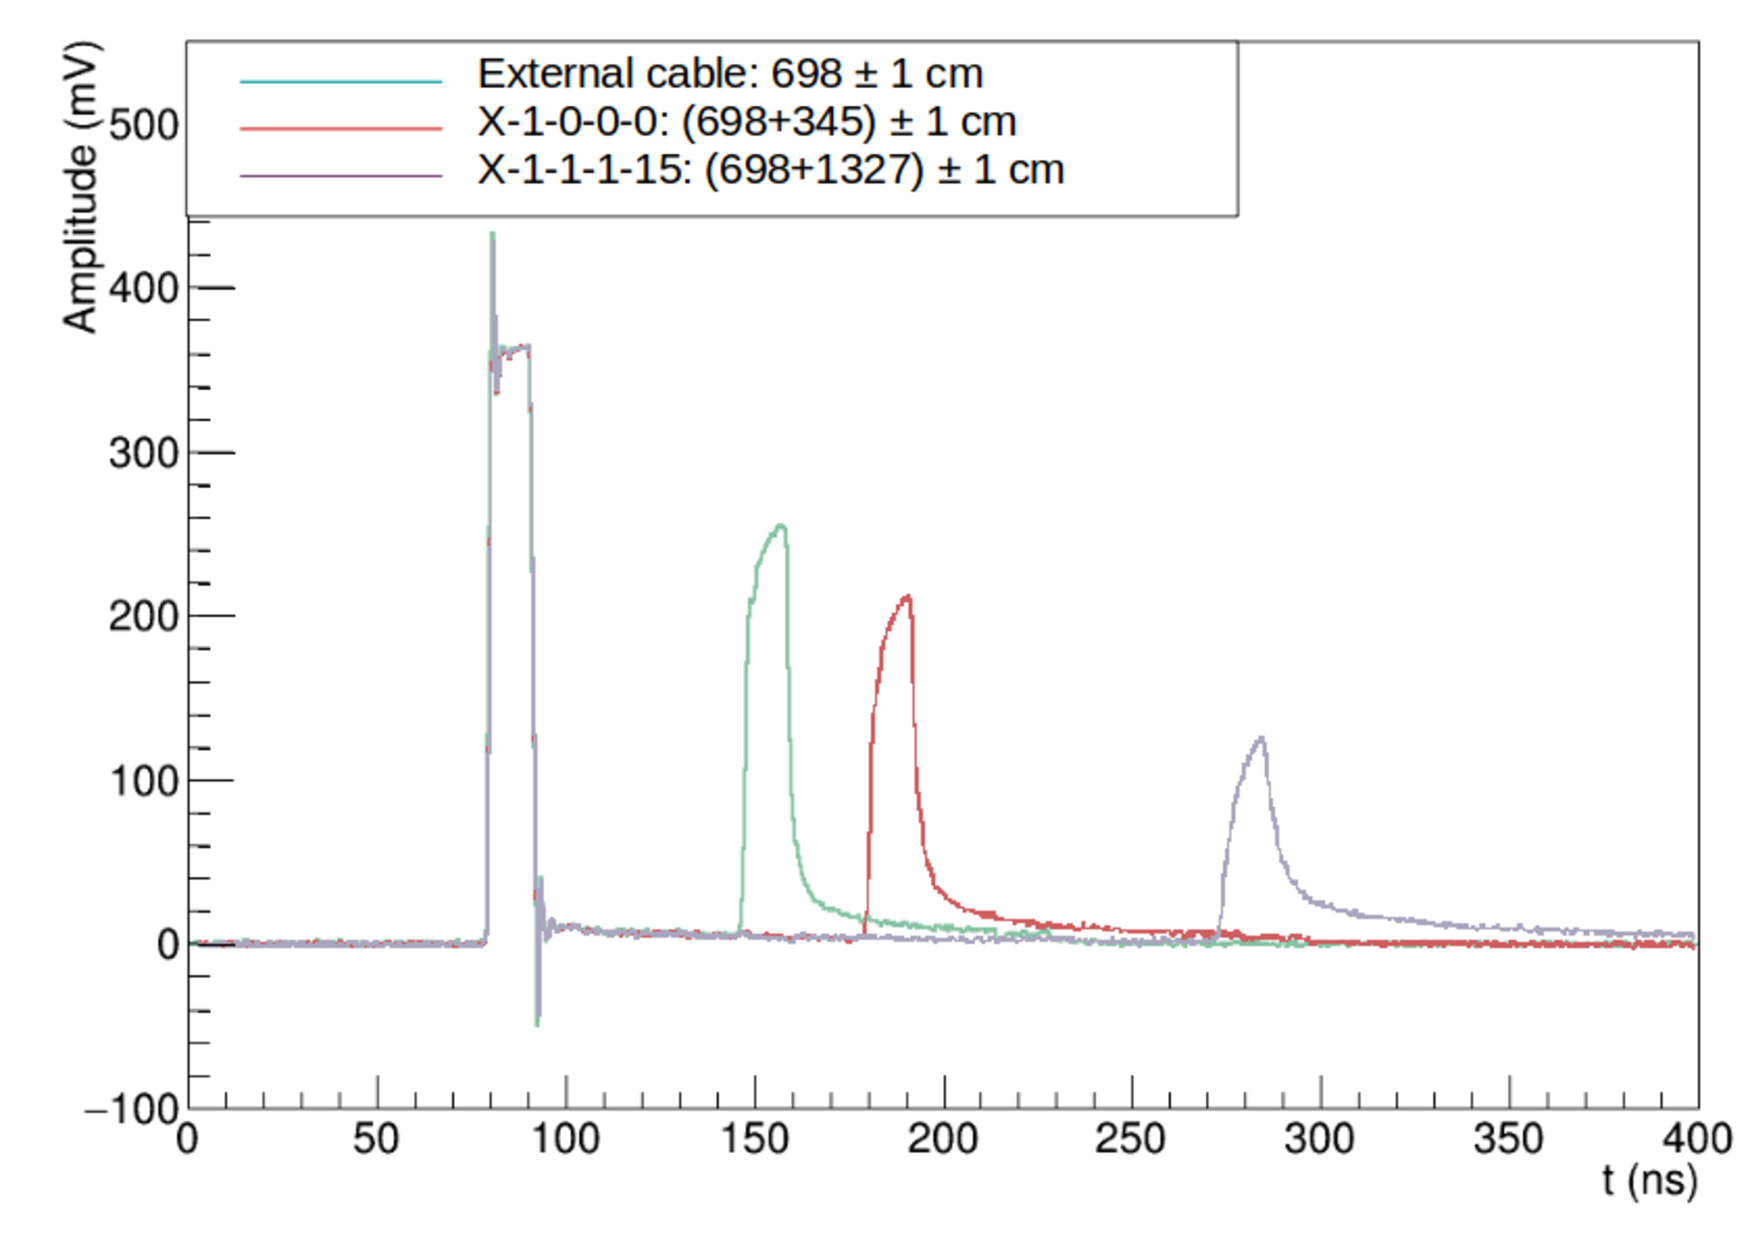
\includegraphics[width=10cm]{commissioning/fig_commissioning/length_tests.pdf}
  \label{fig:cable_lengths}
  \caption{First and back pulses for a $698 \pm 1$ cm cable (green), a $1043 \pm 1$ cm cable (red) and a $2025 \pm 1$ cm cable (grey).}
\end{figure}
